%!TEX program = xelatex

% -----------------------------------------------------------------------------
% ------------------------------- PREAMBLE ------------------------------------
% -----------------------------------------------------------------------------

\documentclass[english]{scrartcl}

\title{An Information Lens on Demographic Diversity} % work on this
\author{\emph{Phil Chodrow}}
\date{\emph{\today}}

\usepackage{pc_writeup}
\usepackage{pc_math}
\usepackage{csvsimple}
\usepackage[colorinlistoftodos]{todonotes}

% -----------------------------------------------------------------------------
% --------------------------------- BODY --------------------------------------
% -----------------------------------------------------------------------------

\begin{document}
\setkomafont{disposition}{\mdseries\rmfamily}

\maketitle

\abstract{}

\section{Introduction} \label{sec:intro}
	\begin{itemize}
		\item While many measures are available for the measurement of spatial diversity, we are not aware of quantitative methods for \emph{identifying} spatial structure. 
		\item We endorse an information-theoretic approach to the study of diversity and segregation. In supporting this approach, we make two main contributions: 
		\begin{itemize}
			\item First, we argue that a simple suite of information measures -- entropy, mutual information, and local information -- intuitively measure global diversity, spatial unevenness, and spatial exposure. The mean local information is novel, and we develop some of its useful properties. This triplet of information measures readily lends itself to quantifying dimensions of segregation within and between cities. 
			\item Measures such as those we develop above can be viewed as measuring different kinds of sociospatial structure. To our knowledge, no such analysis methods have been proposed for \emph{identifying} that structure. Building on our information methods, we develop an algorithm for clustering urban areas into regions whose demographics are near constant in space. The result allows the analyst to both easily visualize spatial patterns of difference and conduct analysis using a natural partition of urban space. 
		\end{itemize}
	\end{itemize}
\section{Lit Review, Previous Work. Why our problem is new.} \label{sec:previous}
	Core points: 
	\begin{itemize}
		\item Previous work is missing unification
		\item Previous work is missing a practical component: how do you compute and learn about urban structure with it? 
	\end{itemize}

\section{Segregation and Information} \label{sec:information}
	Information measures quantify structure through an epistemic framework. The core insight is that systemic structure enables \emph{prediction}, while systemic variability can make such prediction difficult. Two systemic features are related when knowledge of one enables better prediction of the other. 

	We can formalize the idea of prediction quality by considering the following ``guessing game.'' We discuss the weather, and I ask you to give me a \emph{predictive distribution} on the question of whether or not it will rain tomorrow; e.g. ``70\% yes, 30\% no.'' Call this predictive distribution $p$. Tomorrow evening I give you a reward $R(p,Z)$ based on your predictive distribution $p$ and the observed outcome $Z$. For our game to be a true ``guessing game,'' we might expect the reward function $R$ to possess the following intuitive properties: 
	\begin{enumerate}
		\item \textbf{Honesty:} The reward scheme $R$ encourages you to report your true beliefs about the rain.
		\item \textbf{Fairness:} Your reward $R(p,Z)$ you receive depends only on the observed outcome, not ``what could have happened.''
		\item \textbf{Smoothness:} Your reward increases smoothly as a function of the probability you assigned to the observed outcome. 
	\end{enumerate}
	It is possible to show (see e.g. \cite{Cover1991}) that these properties uniquely determine the logarithmic reward function $R(p,Z) = \log p(Z)$ up to an affine transformation. This logarithmic reward is the fundamental unit of information-theoretic analysis. It is customary to focus on the \emph{loss function} $L(p,Z) = - R(p,Z)$. Large loss corresponds to poor prediction. Systemic structure is present when knowledge of a system feature enables us to decrease the loss in such a guessing game. 

	\begin{figure}
		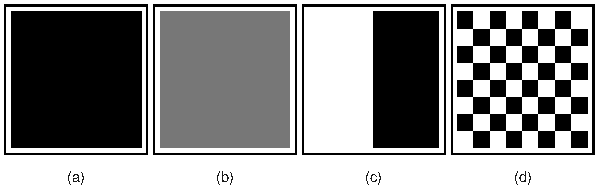
\includegraphics[width=\textwidth]{figs/checkerboard.pdf}
		\caption{Information and the checkerboard}. \label{fig:checkerboard}
	\end{figure}

	\subsection{Entropy and Global Diversity}

		As an introductory example, consider the following guessing game: I pick a person at random from a city, and ask you to assign a predictive distribution on their race $Y$, where $Y$ takes possible values in the alphabet  $\mathcal{Y} = \{\text{Asian, Black, Hispanic, Other, White}\}$. There is a true distribution $p(Y)$ corresponding to the proportions of each race in the city in question. It is possible to show that your optimal guess is precisely this distribution $p$. The optimal expected loss is 
		\begin{equation}
			\E_Y[L(p,Y)] = -\E_Y[R(p,Y)] = -\E_Y[\log p(Y)] \triangleq H(Y), 
		\end{equation}
		also known as the (Shannon) \emph{entropy} of $p$. 

		The Shannon entropy is a natural measure of the global diversity of a city. When $H(Y)$ is low, guessing a randomly-chosen individual's race is easy. An extreme example of this case is when $H(Y) = 0$; in this case, the true distribution $p(Y)$ is unity for one race and zero for the others; i.e. the city is monoracial. Figure \ref{fig:checkerboard}(a) gives an example of this case in a two-race city. Perfect prediction without loss is possible because this city lacks diversity. On the other hand, when $H(Y)$ is high, guessing a randomly-chosen individual's race is difficult. An extreme example of this case is when $H(Y)$ achieves its maximum value of $\log \abs{\mathcal{Y}}$, in which case each race is represented equally. The cities in Figure \ref{fig:checkerboard}(b)-(d) all have maximum demographic entropy. The underlying distribution gives you grounds on which to add probabilistic weight to one race over another; you may as well roll a fair (five-sided) die. Prediction is difficult because of the city's diversity. 

	\subsection{Mutual Information and Spatial (Un)evenness}

		The authors of \cite{Reardon2004} define spatial evenness as ``the extent to which groups are similarly distributed in residential space.'' \emph{Un}evenness, then, is the extent to which these groups are dissimilarly distributed in space. This physical description has an epistemic analogue: knowing where a resident lives conveys information about their race, in the sense of enabling better prediction. To quantify this intuition, consider two versions of the guessing game above. In the first version, I simply choose a random resident and ask you to guess as before. In the second, I choose a random resident but then tell you their residence. In the presence of unevenness, this will generally enable you to improve your predictions. Let $X$ be a random variable denoting the spatial residence. Then, your expected loss in the first game is still $H(Y)$, and your expected loss in the second is $H(Y|X) \triangleq -\E_{Y}[\log p(Y)|X]$. The \emph{mutual information} $I(X,Y)$ is the predictive improvement associated with my telling you the residence: 
		\begin{equation}
			 I(X,Y) \triangleq H(Y) - H(Y|X)\;.
		\end{equation}
		$H(Y)$ is the expected loss without any knowledge of $X$, while $H(Y|X)$ is the expected loss when you are provided the value of $X$ as well. Since knowing $X$ can only improve prediction, $I(X,Y) \geq 0$. Furthermore, it is possible to show that 
		\begin{equation}
			I(X,Y) = D[p(X,Y)\|p(X)p(Y)]\;,
		\end{equation}
		where 
		\begin{equation}
			D[q\|r] \triangleq \sum_a q(a) \log \frac{q(a)}{r(a)}
		\end{equation}
		is the Kullback-Leibler (KL) divergence of $r$ from $q$. Though not an axiomatic metric, the KL divergence may be viewed as a measure of distance between two distributions. The mutual information $I(X,Y)$ can therefore also be viewed as the distance of the true distribution $p(X,Y)$ from the hypothetical distribution $p(X)p(Y)$ in which the variables $X$ and $Y$ are independent. $I(X,Y)$ therefore measures the degree of dependence between these variables. 

		The author of \cite{Roberto2015a} uses the mutual information $I(X,Y)$ -- which she refers to as the Divergence Index -- as a measure of (un)evenness. To see this within our epistemic framework, $I(X,Y) = 0$, $X$ and $Y$ are independent, indicating that knowing $X$ does not improve your ability to guess $Y$. City (b) in Figure \ref{fig:checkerboard} illustrates this situation; since ``everywhere is the same,'' location knowledge is of no predictive value. If we were playing in City (b), your performance in the second guessing game would then be equal to your performance in the first. Physically, this situation corresponds to perfect evenness: the distribution of races is $p(Y|X)$ is the same at every location $X$. In contrast, when $I(X,Y)$ achieves its maximum value of $H(Y)$, $X$ fully determines $Y$. This situation is illustrated by Figure \ref{fig:checkerboard}(c); if I tell you that a resident lives in the left- or right-hand side of the city, you can guess their race with perfect accuracy. This situation corresponds to one in which $H(Y|X) = 0$, i.e. every location is monoracial, reflecting maximal sociospatial unevenness. 

	\subsection{Spatial Exposure}

		The authors of \cite{Reardon2004} define \emph{spatial exposure} as ``the extent that members of one group encounter members of another group...in their local spatial environments.'' We can construct an epistemic analogue of spatial exposure by considering the following pair of guessing games. In each, I pick a resident at random from a fixed ``local spatial environment'' that we both know. In the first game, I ask you to guess that resident's race directly. In the second, I tell you where \emph{within that environment} the resident lives. If the spatial environment in question is $R$, then your expected loss in the first game is $H(Y|X\in B)$ and in the second $H(Y|X, X\in B)$. The prediction improvement associated with knowing residence within this local environment is 
		\begin{equation}
			I(X,Y | X \in B) = H(Y|X\in B) - H(Y|X, X\in B)\;.
		\end{equation}
		Our core claim is that $I(X,Y|X \in B)$ -- the \emph{local (mutual) information} -- is a measure of spatial exposure \emph{in unevenly distributed populations}. This qualification is important, since in a perfectly even population such as Figure \ref{fig:checkerboard}(b),  $I(X,Y) = 0$ and $I(X,Y|X\in B) = 0$ as well. Consider, however, the two unevenly distributed populations in Figure \ref{fig:checkerboard} (c) and (d). In Figure (c), if we play our two guessing games at a locale entirely within the left- or righthand halfs, the population is locally homogeneous and you can make perfect predictions regardless of the specific residence. Only if we play the game on a locale straddling the middle boundary between the two groups does knowing a resident's specific residence help you to make predictions. If our locale $B$ perfectly straddles the boundary, so that the population proportions are $(\frac{1}{2},\frac{1}{2})$, then we have $H(Y|X\in B) = \log 2$ and $H(Y|X,X\in B) = 0$, so $I(X,Y|X \in B) = \log 2$. 

		This example illustrates that the local information $I(X,Y|X\in B)$ is high when $B$ is an area of demographic transition. When two cities are similarly uneven (similar $I(X,Y)$), a city with more such transitional areas has more exposure between groups, since residents of one area are closer to demographically different residents of another area. To illustrate, the city of Figure \ref{fig:checkerboard}(d) has the same level of spatial unevenness as \ref{fig:checkerboard}(c), but greater spatial exposure. 

		For practical data analysis, it is necessary to understand how the value of $I(X,Y|X \in B)$ depends on the choice of the locale $B$. In particular, we should expect that when using fine-grained data and fine-grained spatial locales, our estimates of $I(X,Y|X \in B)$ should converge, and not vary wildly as we increase the resolution of our analysis. It is possible to prove mathematically that this is the case. The full proof is given in the appendix, but the idea of the proof is illustrative of the nature of the local information. It begins by noting that the local information is zero on areas of constant demographic structure, but achieves high values in transitional areas. In this sense it behaves like a mathematical derivative. Making this precise requires that we postulate a metric space $M$ and a \emph{probability field} $p(Y|X)$, $X \in M$ with the following properties: 
		\begin{enumerate}
		 	\item $p(y|x) > 0$ for all $x \in M$
		 	\item $p(y|x)$ is differentiable as a function of $x$ for all $x \in M$. 
		\end{enumerate}
		The probability field $p(y|x)$ corresponds to an idealization of our data; it can be viewed as an interpolation or approximation to the true data using a smooth curve. 

		Define $I_r(x_0)$ to be the local information in a locale of radius $r$ around the point $x_0$:
		\begin{equation}
			I_r(x_0) = I(X,Y| \norm{X - x_0}^2 \leq r^2). 
		\end{equation}
		We may view $r$ as the resolution of our analysis. Under the stated conditions, the following approximation relationship holds: 
		\begin{equation}
			\lim_{r \rightarrow 0} \frac{I_r(x_0)}{r^2} = \frac{1}{4} \text{tr } J_Y(x_0), \label{eq:fisher_approx}
		\end{equation}
		where $J_Y(x_0)$ is the \emph{Fisher information in $Y$ about $x_0$}. $J_Y(x_0)$ is a matrix defined by the formula
		\begin{equation}
			J_Y(x_0) \triangleq \E_Y\left[\nabla_x \log p(Y|x) \left(\nabla_x \log p(Y|x)\right)^T \right]\;. 
		\end{equation}
		The trace $\text{tr }J_Y(x_0)$ of $J_Y(x_0)$ is simply the sum of the diagonal entries of $J_Y(x_0)$. 

		Equation \eqref{eq:fisher_approx} implies that, for small $r$, the local information (when normalized by $r^2$) is approximately a constant that is independent of $r$. Furthermore, that constant is related to the derivatives of the probability field $p(Y|X)$. We can make this relationship more explicit by noting that 
		\begin{equation}
			\text{tr }J_Y(x_0) = \E_Y\left[\norm{\nabla_x \log p(Y|x_0)}^2\right]\;, \label{eq:derivative}
		\end{equation}
		which together with \eqref{eq:fisher_approx} shows that $I_r(x_0)$ is proportional to the mean magnitude of the derivative of $p(Y|X)$ evaluated at $x = x_0$.

		In the idealized mathematical framework, we may define the \emph{mean local information} as the average value of the trace of the Fisher information: 
		\begin{equation}
			J(X,Y) \triangleq \E_X[\text{tr } J_Y(X)].
		\end{equation}
		Using the relationship \eqref{eq:derivative}, we can recognize $J(X,Y)$ as the total variation of $\log p(Y|X)$ with respect to the probability measure induced by $X$. Intuitively, this is the average ``curviness'' of the field $p(Y|X)$. 

		It is simple to adopt this measure $J(X,Y)$ for practical data analysis. The procedure is as follows: 
		\begin{enumerate}
		 	\item Partition the city under analysis into spatial locales $\{B_i\}$.
		 	\item Compute the local information $I(X,Y|X \in B_i)$ for each $i$. 
		 	\item Average the results, weighted by the population of each $B_i$. 
		\end{enumerate} 
		The explicit formula is 
		\begin{equation}
			J(X,Y) = \sum_i p(X \in B_i) I(X,Y|X \in B_i). \label{eq:formula}
		\end{equation}

	\subsection{Illustrations}
		% \subsubsection{Comparative Analysis: Detroit and Philadelphia}
			To illustrate these methods, we use them to compare the cities of Philadelphia and Detroit. Our data is blockgroup-level demographics from the American Community Survey \cite{CensusRace}. As we show, computing $H(Y)$, $I(X,Y)$, and $J(X,Y)$ together highlights similarities and differences between these cities. 
			% \todo{We need to generate a nice summary plot here and then fill this section in.}
			\begin{figure}
				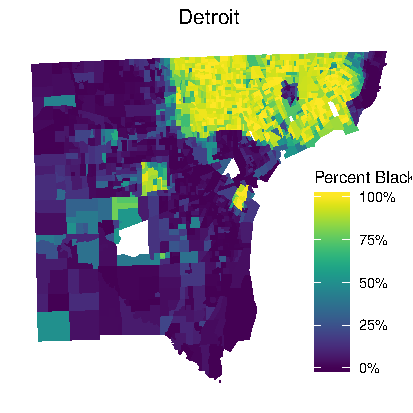
\includegraphics[width = .5\textwidth]{figs/Detroit_percent_black.pdf}
				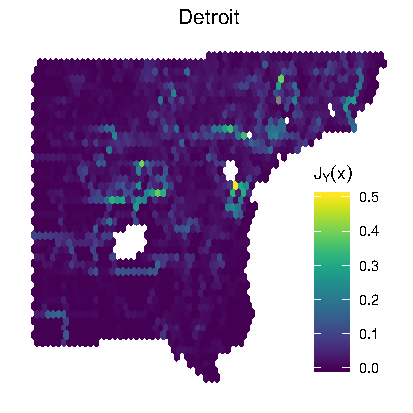
\includegraphics[width = .5\textwidth]{figs/Detroit_grid.pdf} \\
				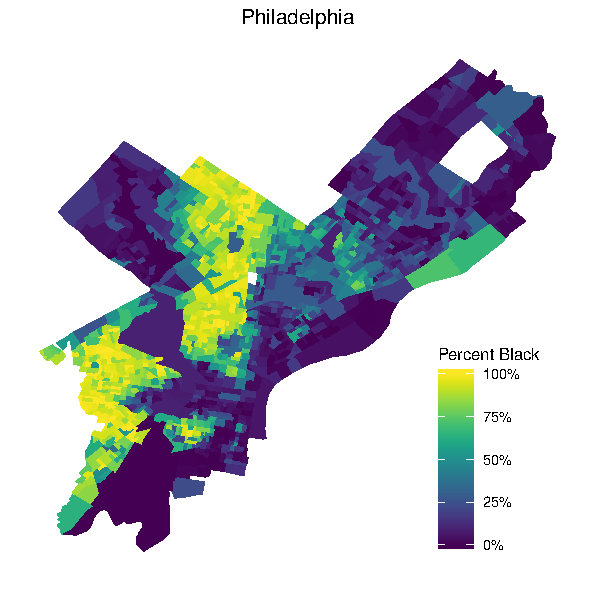
\includegraphics[width = .5\textwidth]{figs/Philadelphia_percent_black.pdf}
				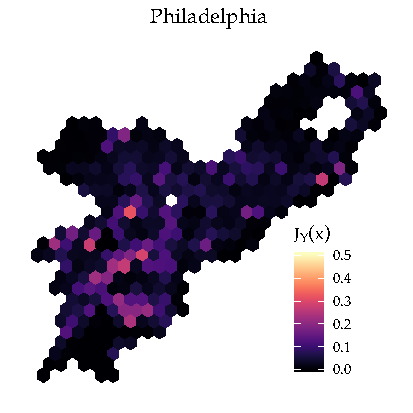
\includegraphics[width = .5\textwidth]{figs/Philadelphia_grid.pdf} \\

				\centering
				\begin{tabular}{l | c c c c}
					\bfseries City & Percent Black & $H(Y)$ & $I(X,Y)$ & $J(X,Y)$  \\\hline
					\csvreader[late after line=\\]{figs/comparative_summary.csv}{}
					{\csvcoli & \csvcolii & \csvcoliii & \csvcoliv & \csvcolv}
				\end{tabular}

				\caption{Spatial analysis of racial diversity in Detroit (top) and Philadelphia (middle). Left: Percentage of black residents in Detroit (left) and Philadelphia (right). Right: Hexgrid of spatial resolution 1km imposed over each city, shaded by the value of $I(X,Y | X \in B_i)$. Bottom: Numerical summary, including the three information measures.} \label{fig:detroit_philly}
			\end{figure}

		% \subsubsection{Comparative Diversity Profiles}
			% \todo{Is there a fun way to explore the density point? E.g. figure out people per ``neighborhood'' in some way? Think about what I would want the analysis here to be.}

			We can achieve a broader picture by comparing $I(X,Y)$ and $J(X,Y)$ across a range of American cities, as we do in Figure \ref{fig:mutual_fisher}. The two measures $I(X,Y)$ and $J(X,Y)$ provide an intuitive sorting of major cities. Cities with small numbers of large, monoracial regions such as Atlanta and Detroit are sorted toward the bottom right while cities with more complicated patchworks of demographic variation like Philadelphia and New York are sorted toward the top right. 

			\begin{figure}
				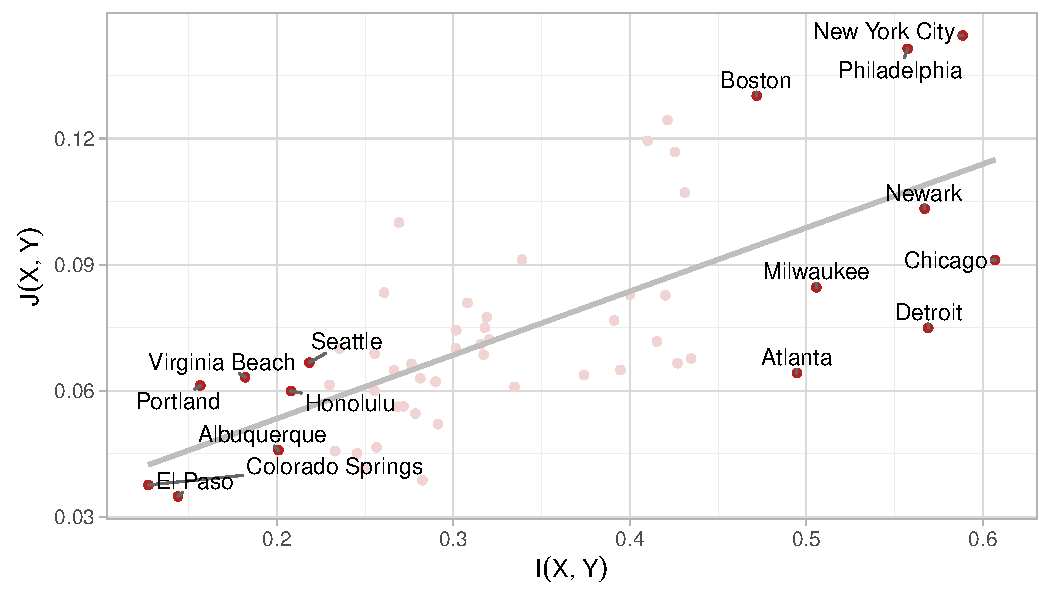
\includegraphics[width=\textwidth]{figs/mutual_fisher.pdf}
				\caption{Comparative global diversity measures in major U.S. cities. Cities toward the bottom left are relatively spatially even. Cities toward the bottom right like Detroit and Atlanta are the most classically ``segregated'', with large, starkly separated monoracial regions. Cities toward the top right like Philadelphia and New York are complex ``patchworks'' of different, smaller regions.} \label{fig:mutual_fisher}
			\end{figure}

			\todo{Optional: plot of $J$ vs. density in here, but probably only if we can think of more to say, possibly a follow-up analysis.}	

\section{Identifying Sociospatial Structure} \label{sec:id}

	We can view $H(Y)$, $I(X,Y)$, and $J(X,Y)$ as measures of the presence of sociospatial structure. It is somewhat unsatisfying to simply measure this structure without actually identifying it, since identifying this structure is of direct application in sociological data analysis. In this section, we use information-theoretic techniques to construct a procedure for finding subregions within cities that capture high-level demographic trends. 

	A useful place to start is with the property of ``additive spatial decomposition'' \cite{Reardon2004}. A diversity measure satisfies additive spatial decomposition when, if spatial units are aggregated into groups, the measure can be expressed as a sum of a ``within group'' term expressing variability within aggregations, and a ``between group'' term expressing variability across aggregations. The mutual information $I(X,Y)$ satisfies this property due to the following information-theoretic identity. Let $C$ be a random variable with the property that $H(C|X) = 0$; i.e. $X$ completely determines $C$. We can think of $C$ as group labels for the spatial locations $X$. Then, the chain rule of information implies that 
	\begin{equation}
		I(X,Y) = \underbrace{I(C,Y)}_{\text{between-group}} + \underbrace{I(X,Y|C)}_{\text{within-group}}. \label{eq:chain_rule}
	\end{equation}
	Equation \eqref{eq:chain_rule} expresses the following intuitive information decomposition: the information you have if I tell you first a resident's approximate residence $C$ and subsequently their exact residence $X$ is just the same as the information you would have if I simply told you $X$ directly. 

	Equation \eqref{eq:chain_rule} also motivates a natural algorithm for identifying sociospatial structure. The core idea is that a clustering $C$ is ``good'' when it captures most of the intrinsic information in the system in the between-groups term $I(C,Y)$. This idea is analogous to between-group sum-of-squares maximization in classical ANOVA methods. We therefore seek to maximize $I(C,Y)$. In full generality, this is a challenging discrete optimization problem that may not be computationally tractable. We can, however, construct a ``greedy'' algorithm which, though suboptimal, leads to satisfactory results. At each stage of the algorithm, we consider the problem of choosing a pair of locales $\{i*, j*\}$ to aggregate together. A good choice of locales leads to minimal information loss, which we may quantify as follows. The mutual information may also be written: 
	\begin{align}
	 	I(X,Y) &= \sum_k p(X = k) D[p(Y|X = k\|p(Y)] 
	\end{align} 
	The contribution of locale $i$ to this sum is 
	\begin{align}
		I_{i}(X,Y) &\triangleq \sum_{k \in \{i\}} p(X = i)D[p(Y|X = i\|p(Y)] 
	\end{align}
	If we replace $i$ and $j$ with an aggregated local $i\cup j$, its contribution to the mutual information is 
	\begin{align}
		I_{i\cup j}(X,Y) = p(X \in \{i,j\}) D[p(Y|X \in \{i,j\}) \| p(Y)]\;.
	\end{align}
	The  loss associated with aggregating $i$ and $j$ is the difference between individual contributions and their aggregated contribution:
	\begin{align}
		d(i,j) \triangleq I_{i}(X,Y) + I_{j}(X,Y) - I_{i \cup j}(X,Y).  
	\end{align}
	Like the KL divergence $D$, the function $d$ can be viewed as a measure of distance between probability distributions $p(Y|X = i)$ and $p(Y|X = j)$. Unlike the KL divergence, $d$ is symmetric in $i$ and $j$; it is not a true metric because it does not satisfy the triangle inequality. It can nevertheless be used to motivate a form of agglomerative hierarchical clustering, where at each phase of the algorithm we compute 
	\begin{equation}
		(i^*m, j^*) = \argmin_{i \text{neighbors} j} \; d(i,j)\;
	\end{equation}
	and combine $i^*$ and $j^*$ into a single new group. We repeat this procedure until only one group remains. The optimizatin over $i$ and $j$ ensures that the groupings so defined approximate maximum between-group information partitions, and the constraint that $i$ must neighbor $j$ ensures that the structure so determined is spatially contiguous. Since this is a greedy algorithm, it possesses no guarantees of solution optimality, but in practice its performance leads to intuitive, demographically-coherent regions. 

	To demonstrate the power of this approach for data analysis, 



	\begin{itemize}
		\item Construct the algorithm. 
		\item Prove the triangle inequality
		\item Show algorithm results for one or two cities; show how knowing the clusters can lead to neat data analysis. 
		\item Relate algorithmic performance to suite of information measures above. Note that $J$ measures the ``natural fault lines'' where we would expect the algorithm to segment.  
	\end{itemize}

\section{Discussion} \label{sec:discussion}
BLAH BLAH BLAH
% \bibliography{/Users/phil/bibs/library.bib}{}
% \bibliographystyle{plain}


% TODO: 

% - Think about whether we should also be looking at pairwise group exposure metrics? Is there an information-theoretic version of this? Maybe the information-loss associated with aggregating those two groups, that's not a bad guess. 


\end{document}